\documentclass[twoside]{book}

% Packages required by doxygen
\usepackage{fixltx2e}
\usepackage{calc}
\usepackage{doxygen}
\usepackage[export]{adjustbox} % also loads graphicx
\usepackage{graphicx}
\usepackage[utf8]{inputenc}
\usepackage{makeidx}
\usepackage{multicol}
\usepackage{multirow}
\PassOptionsToPackage{warn}{textcomp}
\usepackage{textcomp}
\usepackage[nointegrals]{wasysym}
\usepackage[table]{xcolor}

% Font selection
\usepackage[T1]{fontenc}
\usepackage[scaled=.90]{helvet}
\usepackage{courier}
\usepackage{amssymb}
\usepackage{sectsty}
\renewcommand{\familydefault}{\sfdefault}
\allsectionsfont{%
  \fontseries{bc}\selectfont%
  \color{darkgray}%
}
\renewcommand{\DoxyLabelFont}{%
  \fontseries{bc}\selectfont%
  \color{darkgray}%
}
\newcommand{\+}{\discretionary{\mbox{\scriptsize$\hookleftarrow$}}{}{}}

% Page & text layout
\usepackage{geometry}
\geometry{%
  a4paper,%
  top=2.5cm,%
  bottom=2.5cm,%
  left=2.5cm,%
  right=2.5cm%
}
\tolerance=750
\hfuzz=15pt
\hbadness=750
\setlength{\emergencystretch}{15pt}
\setlength{\parindent}{0cm}
\setlength{\parskip}{3ex plus 2ex minus 2ex}
\makeatletter
\renewcommand{\paragraph}{%
  \@startsection{paragraph}{4}{0ex}{-1.0ex}{1.0ex}{%
    \normalfont\normalsize\bfseries\SS@parafont%
  }%
}
\renewcommand{\subparagraph}{%
  \@startsection{subparagraph}{5}{0ex}{-1.0ex}{1.0ex}{%
    \normalfont\normalsize\bfseries\SS@subparafont%
  }%
}
\makeatother

% Headers & footers
\usepackage{fancyhdr}
\pagestyle{fancyplain}
\fancyhead[LE]{\fancyplain{}{\bfseries\thepage}}
\fancyhead[CE]{\fancyplain{}{}}
\fancyhead[RE]{\fancyplain{}{\bfseries\leftmark}}
\fancyhead[LO]{\fancyplain{}{\bfseries\rightmark}}
\fancyhead[CO]{\fancyplain{}{}}
\fancyhead[RO]{\fancyplain{}{\bfseries\thepage}}
\fancyfoot[LE]{\fancyplain{}{}}
\fancyfoot[CE]{\fancyplain{}{}}
\fancyfoot[RE]{\fancyplain{}{\bfseries\scriptsize Generated by Doxygen }}
\fancyfoot[LO]{\fancyplain{}{\bfseries\scriptsize Generated by Doxygen }}
\fancyfoot[CO]{\fancyplain{}{}}
\fancyfoot[RO]{\fancyplain{}{}}
\renewcommand{\footrulewidth}{0.4pt}
\renewcommand{\chaptermark}[1]{%
  \markboth{#1}{}%
}
\renewcommand{\sectionmark}[1]{%
  \markright{\thesection\ #1}%
}

% Indices & bibliography
\usepackage{natbib}
\usepackage[titles]{tocloft}
\setcounter{tocdepth}{3}
\setcounter{secnumdepth}{5}
\makeindex

% Custom commands
\newcommand{\clearemptydoublepage}{%
  \newpage{\pagestyle{empty}\cleardoublepage}%
}

\usepackage{caption}
\captionsetup{labelsep=space,justification=centering,font={bf},singlelinecheck=off,skip=4pt,position=top}

%===== C O N T E N T S =====

\begin{document}

% Titlepage & ToC
\pagenumbering{roman}
\begin{titlepage}
\vspace*{7cm}
\begin{center}%
{\Large V\+D\+S\+Project }\\
\vspace*{1cm}
{\large Generated by Doxygen 1.8.11}\\
\end{center}
\end{titlepage}
\clearemptydoublepage
\tableofcontents
\clearemptydoublepage
\pagenumbering{arabic}

%--- Begin generated contents ---
\chapter{Class Index}
\section{Class List}
Here are the classes, structs, unions and interfaces with brief descriptions\+:\begin{DoxyCompactList}
\item\contentsline{section}{{\bf Class\+Project\+::\+B\+D\+D\+\_\+\+Node} \\*Typedef struct \doxyref{B\+D\+D\+\_\+\+Node}{p.}{structClassProject_1_1BDD__Node} }{\pageref{structClassProject_1_1BDD__Node}}{}
\item\contentsline{section}{{\bf Class\+Project\+::\+B\+D\+D\+Comparer} \\*Typedef struct \doxyref{B\+D\+D\+Comparer}{p.}{structClassProject_1_1BDDComparer} }{\pageref{structClassProject_1_1BDDComparer}}{}
\item\contentsline{section}{{\bf Class\+Project\+::\+Manager} \\*\doxyref{Manager}{p.}{classClassProject_1_1Manager} Class }{\pageref{classClassProject_1_1Manager}}{}
\item\contentsline{section}{{\bf Class\+Project\+::\+Manager\+Interface} }{\pageref{classClassProject_1_1ManagerInterface}}{}
\end{DoxyCompactList}

\chapter{Class Documentation}
\section{Class\+Project\+:\+:Manager\+Interface Class Reference}
\label{classClassProject_1_1ManagerInterface}\index{Class\+Project\+::\+Manager\+Interface@{Class\+Project\+::\+Manager\+Interface}}
Inheritance diagram for Class\+Project\+:\+:Manager\+Interface\+:\begin{figure}[H]
\begin{center}
\leavevmode
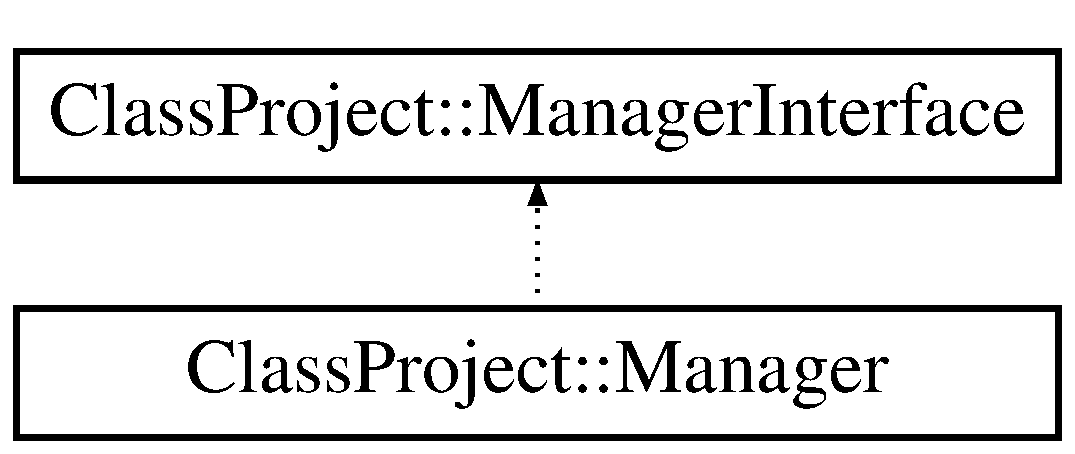
\includegraphics[height=2.000000cm]{classClassProject_1_1ManagerInterface}
\end{center}
\end{figure}
\subsection*{Public Member Functions}
\begin{DoxyCompactItemize}
\item 
virtual B\+D\+D\+\_\+\+ID {\bfseries create\+Var} (const std\+::string \&label)=0\label{classClassProject_1_1ManagerInterface_ab101acd3fbe6a5e29973d88f9862b8b4}

\item 
virtual const B\+D\+D\+\_\+\+ID \& {\bfseries True} ()=0\label{classClassProject_1_1ManagerInterface_a104d0e8bcbd81eb501b66db6e24d1f63}

\item 
virtual const B\+D\+D\+\_\+\+ID \& {\bfseries False} ()=0\label{classClassProject_1_1ManagerInterface_a98d18e1bc840fd664af015facfdcf690}

\item 
virtual bool {\bfseries is\+Constant} (const B\+D\+D\+\_\+\+ID f)=0\label{classClassProject_1_1ManagerInterface_a0edd879f6ecae7bc5f84a2d55373d977}

\item 
virtual bool {\bfseries is\+Variable} (const B\+D\+D\+\_\+\+ID x)=0\label{classClassProject_1_1ManagerInterface_a6eaaec7cbf8826198e490313ccb8f22a}

\item 
virtual B\+D\+D\+\_\+\+ID {\bfseries top\+Var} (const B\+D\+D\+\_\+\+ID f)=0\label{classClassProject_1_1ManagerInterface_ae2c645f859bcc7be3376d478f01eb045}

\item 
virtual B\+D\+D\+\_\+\+ID {\bfseries ite} (const B\+D\+D\+\_\+\+ID i, const B\+D\+D\+\_\+\+ID t, const B\+D\+D\+\_\+\+ID e)=0\label{classClassProject_1_1ManagerInterface_a6ea8f9482d86afb4128c52328d9ec11c}

\item 
virtual B\+D\+D\+\_\+\+ID {\bfseries co\+Factor\+True} (const B\+D\+D\+\_\+\+ID f, B\+D\+D\+\_\+\+ID x)=0\label{classClassProject_1_1ManagerInterface_aab8496a0e551abdad99160e152199f4b}

\item 
virtual B\+D\+D\+\_\+\+ID {\bfseries co\+Factor\+False} (const B\+D\+D\+\_\+\+ID f, B\+D\+D\+\_\+\+ID x)=0\label{classClassProject_1_1ManagerInterface_ad749ef1542c5b23bbbce628d6f666fe4}

\item 
virtual B\+D\+D\+\_\+\+ID {\bfseries co\+Factor\+True} (const B\+D\+D\+\_\+\+ID f)=0\label{classClassProject_1_1ManagerInterface_a4a1880d2245af9130646232551940949}

\item 
virtual B\+D\+D\+\_\+\+ID {\bfseries co\+Factor\+False} (const B\+D\+D\+\_\+\+ID f)=0\label{classClassProject_1_1ManagerInterface_a308c99661ad02f407d6f2b0af6230e80}

\item 
virtual B\+D\+D\+\_\+\+ID {\bfseries and2} (const B\+D\+D\+\_\+\+ID a, const B\+D\+D\+\_\+\+ID b)=0\label{classClassProject_1_1ManagerInterface_af914326d34a1ed42710f7b11e5baf010}

\item 
virtual B\+D\+D\+\_\+\+ID {\bfseries or2} (const B\+D\+D\+\_\+\+ID a, const B\+D\+D\+\_\+\+ID b)=0\label{classClassProject_1_1ManagerInterface_a8dbfde761b1e94d1f222b4d27f3c6fbc}

\item 
virtual B\+D\+D\+\_\+\+ID {\bfseries xor2} (const B\+D\+D\+\_\+\+ID a, const B\+D\+D\+\_\+\+ID b)=0\label{classClassProject_1_1ManagerInterface_a2b2c4948ef41ddb1036289cd07dac156}

\item 
virtual B\+D\+D\+\_\+\+ID {\bfseries neg} (const B\+D\+D\+\_\+\+ID a)=0\label{classClassProject_1_1ManagerInterface_a57d34af3121dcf5366d22ecf792f05a0}

\item 
virtual B\+D\+D\+\_\+\+ID {\bfseries nand2} (const B\+D\+D\+\_\+\+ID a, const B\+D\+D\+\_\+\+ID b)=0\label{classClassProject_1_1ManagerInterface_aaf6e357d680613e449d3ea958c9abba1}

\item 
virtual B\+D\+D\+\_\+\+ID {\bfseries nor2} (const B\+D\+D\+\_\+\+ID a, const B\+D\+D\+\_\+\+ID b)=0\label{classClassProject_1_1ManagerInterface_a312d9865eae2d6355e17855cba78bc78}

\item 
virtual std\+::string {\bfseries get\+Top\+Var\+Name} (const B\+D\+D\+\_\+\+ID \&root)=0\label{classClassProject_1_1ManagerInterface_afde45b2065361dfa6e61c1c7bc3fc1b4}

\item 
virtual void {\bfseries find\+Nodes} (const B\+D\+D\+\_\+\+ID \&root, std\+::set$<$ B\+D\+D\+\_\+\+ID $>$ \&nodes\+\_\+of\+\_\+root)=0\label{classClassProject_1_1ManagerInterface_ab460e331ffdb85d4128574b3aae72c1e}

\item 
virtual void {\bfseries find\+Vars} (const B\+D\+D\+\_\+\+ID \&root, std\+::set$<$ B\+D\+D\+\_\+\+ID $>$ \&vars\+\_\+of\+\_\+root)=0\label{classClassProject_1_1ManagerInterface_ab94feabca2125d334e542e502ae0186d}

\item 
virtual size\+\_\+t {\bfseries unique\+Table\+Size} ()=0\label{classClassProject_1_1ManagerInterface_a85cac80444b26e5b80eb96b9f1231c0e}

\end{DoxyCompactItemize}


The documentation for this class was generated from the following file\+:\begin{DoxyCompactItemize}
\item 
/import/home/vdscp04/\+Luiz/vdscp\+\_\+04/src/Manager\+Interface.\+h\end{DoxyCompactItemize}

%--- End generated contents ---

% Index
\backmatter
\newpage
\phantomsection
\clearemptydoublepage
\addcontentsline{toc}{chapter}{Index}
\printindex

\end{document}
